\documentclass[document.tex]{subfiles}
\begin{document}

\chapter{Hyperspectral Imaging}
\section{Introduction}
The most significant recent breakthrough in remote sensing has been the development of
hyperspectral sensors and software to analyze the resulting image data\cite{3}. Fifteen years ago only spectral remote sensing experts had access to hyperspectral images or software tools to take advantage of such images. Over the past decade hyperspectral image analysis
has matured into one of the most powerful and fastest growing technologies in the field
of remote sensing. The "hyper" in hyperspectral means "over" as in "too many" and
refers to the large number of measured wavelength bands. Hyperspectral images are
spectrally overdetermined, which means that they provide ample spectral information to
identify and distinguish spectrally unique materials. Hyperspectral imagery provides the
potential for more accurate and detailed information extraction than possible with any
other type of remotely sensed data.
\section{Spectral Image Basics}
\noindent To understand the advantages of hyperspectral imagery, it may help to first review some
basic spectral remote sensing concepts. You may recall that each photon of light has
a wavelength determined by its energy level. Light and other forms of electromagnetic
radiation are commonly described in terms of their wavelengths. For example, visible
light has wavelengths between 0.4 and 0.7 microns, while radio waves have wavelengths
greater than about 30 cm (Figure. 2.1).
\begin{figure}[H]
	\begin{center}
		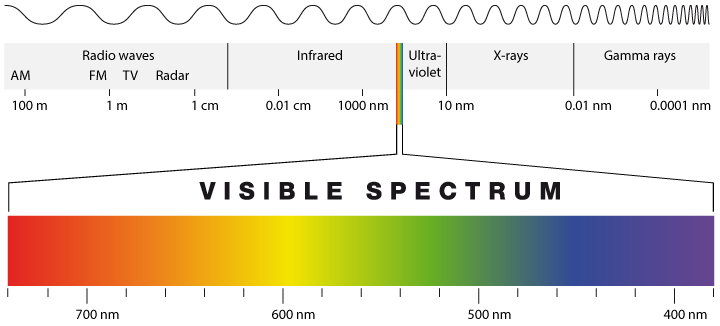
\includegraphics[height=6.0cm]{imgs/Electromagnetic_spectrum.png}
	\end{center}
	\caption{The electromagnetic spectrum}
	\label{fig: The electromagnetic spectrum}
\end{figure}
\noindent Reflectance is the percentage of the light hitting a material that is then reflected by
that material (as opposed to being absorbed or transmitted). A reflectance spectrum
shows the reflectance of a material measured across a range of wavelengths (Fig. 2.2).
Some materials will reflect certain wavelengths of light, while other materials will absorb
the same wavelengths. These patterns of reflectance and absorption across wavelengths
can uniquely identify certain materials.
\begin{figure}[H]
	\begin{center}
		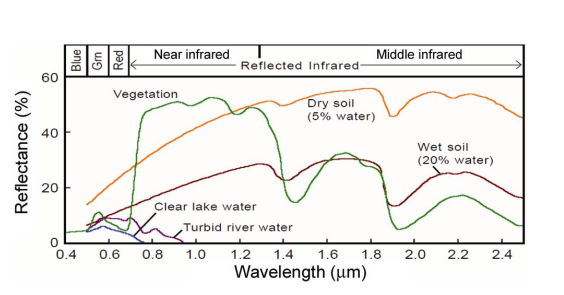
\includegraphics[height=8.0cm]{imgs/Materials.png}
	\end{center}
	\caption{Reflectance spectra for several common Earth surface materials}
	\label{fig: Reflectance spectra for several common Earth surface materials}
\end{figure}

\begin{figure}[H]
	\begin{center}
		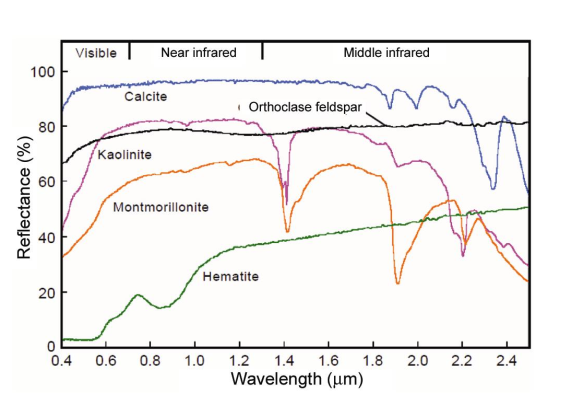
\includegraphics[height=8.0cm]{imgs/Minerals.png}
	\end{center}
	\caption{Reflectance spectra for important minerals}
	\label{fig: Reflectance spectra for important minerals}
\end{figure}
\noindent Field and laboratory spectrometers usually measure reflectance at many narrow,
closely spaced wavelength bands, so that the resulting spectra appear to be continuous curves (Fig. 2.2). When a spectrometer is used in an imaging sensor, the resulting
images record a reflectance spectrum for each pixel in the image (Fig. 2.4).
\begin{figure}[H]
	\begin{center}
		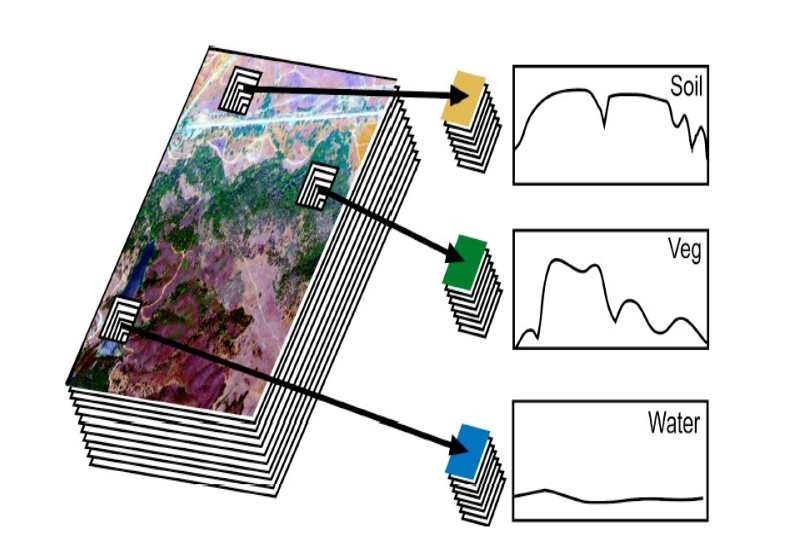
\includegraphics[height=8.0cm]{imgs/Hyperspectral_imagery.png}
	\end{center}
	\caption{The concept of hyperspectral imagery. Image measurements are made at
		many narrow contiguous wavelength bands, resulting in a complete spectrum for each
		pixel.}
	\label{fig: Hyperspectral imagery}
\end{figure}
\section{Hyperspectral Data}
Most multispectral imagers (e.g., Landsat, SPOT, AVHRR) measure radiation reflected
from a surface at a few wide, separated wavelength bands. Most hyperspectral
imagers, on the other hand, measure reflected radiation at a series of narrow
and contiguous wavelength bands. When we look at a spectrum for one pixel in a
hyperspectral image, it looks very much like a spectrum that would be measured in a
spectroscopy laboratory. This type of detailed pixel spectrum can provide much
more information about the surface than a multispectral pixel spectrum.
\begin{figure}[H]
	\begin{center}
		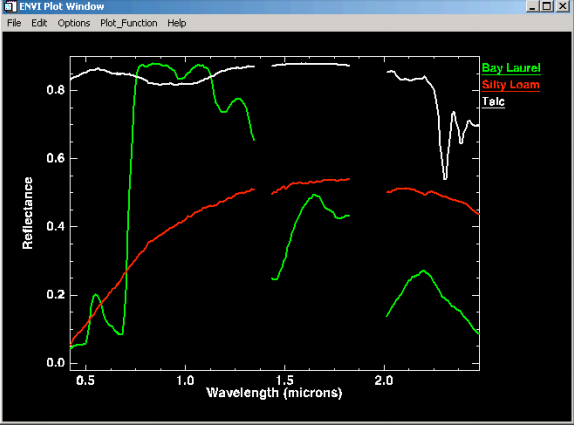
\includegraphics[height=8.0cm]{imgs/Atmosphere.png}
	\end{center}
	\caption{Reflectance spectra of the three materials as they would appear to the hyperspectral AVIRIS sensor. The gaps in the spectra are wavelength ranges at which the atmosphere absorbs so much light that no reliable signal is received from the surface.}
	\label{fig: Effect of atmospheric absorbtion over hyperspectral data}
\end{figure}
\noindent Although most hyperspectral sensors measure hundreds of wavelengths, it is not the
number of measured wavelengths that defines a sensor as hyperspectral. Rather it is the
narrowness and contiguous nature of the measurements. For example, a sensor that
measured only 20 bands could be considered hyperspectral if those bands were
contiguous and, say, 10 nm wide. If a sensor measured 20 wavelength bands that were,
say, 100 nm wide, or that were separated by non-measured wavelength ranges, the sensor
would no longer be considered hyperspectral.
\noindent Standard multispectral image classification techniques were generally developed to
classify multispectral images into broad categories. Hyperspectral imagery provides an
opportunity for more detailed image analysis. For example, using hyperspectral data,
spectrally similar materials can be distinguished\cite{6} and sub-pixel scale information can be extracted. To fulfill this potential, new image processing techniques have been
developed.
\section{Sensors}
The Landsat earth resources satellite system was the first designed to provide near
global coverage of the earth’s surface on a regular and predictable basis.
The first three Landsats had identical orbit characteristics, as summarised in
Table A.4. The orbits were near polar and sun synchronous – i.e., the orbital plane
precessed about the earth at the same rate that the sun appears to move across the
face of the earth. In this manner data was acquired at about the same local time on
every pass.
\begin{table}[H]
	\caption{Landsat 1, 2, 3 orbit characteristics}
	\begin{center}
		\begin{tabularx}{\columnwidth}{|XX|}
			\hline Orbit: & Sun synchronous,near polar and nominal 9:30 am descending equatorial crossing; inclined at about 99$\deg$ to equator\\
			Altitude: & 920km (570 mi)\\
			Period: & 103 min\\
			Repeat Cycle: & 14 orbits per day over 18 days (251 revolutions)\\\hline
		\end{tabularx}
	\end{center}
	\label{tab:Landsat 1, 2, 3 orbit characteristics}
\end{table}

\noindent Most past and current hyperspectral sensors have been airborne, with two
recent exceptions: NASA’s Hyperion sensor on the EO-1 satellite, and the U.S. Air
Force Research Lab’s FTHSI sensor on the MightySat II satellite. Several new spacebased
hyperspectral sensors have been proposed recently. Unlike airborne
sensors, space-based sensors are able to provide near global coverage repeated at regular
intervals. Therefore, the amount of hyperspectral imagery available should increase
significantly in the near future as new satellite-based sensors are successfully launched.
\begin{table}[H]
	\caption{Current and Recent Hyperspectral Sensors and Data Providers}
	\begin{center}
		\begin{tabularx}{\columnwidth}{|X|X|X|X|}
			\hline
			Sensors & Manufacturer & Number of
			Bands &
			Spectral Range\\ \hline
			
			AVIRIS
			(Airborne
			Visible
			Infrared
			Imaging
			Spectrometer) &
			NASA Jet
			Propulsion Lab
			makalu.jpl.nasa.gov/ &
			224 & 0.4 to 2.5 $\mu$m\\ \hline
			
			HYDICE
			(Hyperspectral
			Digital
			Imagery
			Collection
			Experiment) &
			Naval Research Lab & 210 & 0.4 to 2.5 $\mu$m \\ \hline
			
			FTHSI on
			MightySat
			II &
			Air Force Research
			Lab www.vs.afrl.af.mil
			/TechProgs/MightySatII &
			256  & 0.35 to 1.05 $\mu$m \\ \hline
			Hyperion
			on EO- 1 &
			NASA Goddard
			Space Flight Center
			eo1.gsfc.nasa.gov &
			220 & 0.4 to 2.5 $\mu$m\\ \hline
			
			PROBE-
			1 Earth
			Search
			Sciences
			Inc. &
			www.earthsearch .com & 128 & 0.4 to 2.5 $\mu$m\\ \hline
			
			CASI (Compact
			Airborne
			Spectrographic
			Imager) &
			ITRES Research Limited
			www.itres.com
			up to  & 228 & 0.4 to 1.0$\mu$m\\ \hline
		\end{tabularx}
	\end{center}
	\label{tab:Current and Recent Hyperspectral Sensors and Data Providers}
\end{table}
\clearpage
\section{Application of Hyperspectral Image Analysis}
Multi spectral images like Landsat thematic Mapper and SPOT XS produce few broad wavelength bands but the hyperspectral image sensor will produce narrower wavelength bands. These bands can range from 100 to 200 or more. These measurement make it possible to derive continuous spectrum for each image cell, see below image. After sensor is adjusted, terrain and atmospheric condition are applied, then the results is verified against the collected spectrum value to categorize the type of vegetation or minerals or other features. Hyperspectral images contain ton of information, surface information and its spectrum behavior should be understand deeply and how it related to the hyperspectral images. This type of image are finding their importance in different fields as before it was just used for remote sensing application. Here are few applications of hyperspectral images.
\begin{enumerate}
	\item \textbf{Remote Sensing:} In remote sensing technology it is very important to distinguish earth surface features, each features have different spectrum band. Multi spectral satellite can capture image up few bands for example Landsat 7 have 8 bands. But multi spectral imaging satellite can capture earth surface in more than 200 bands which helps scientist to differentiate objects that were not possible in multi spectral imaging because of spectral resolution.
	\item \textbf{Seed Viability Study: }By using the hyperspectral image and plotting the reflectance spectrum one can conclude that whether those seed are viable or not viable. Seed might be looking same through naked eyes but its viability will be trace down by the hyperspectral image.
	\item \textbf{Biotechnology:} Hyperspectral technology has become popular in the biological and medical applications. It is easy and quick to acquire the data that can be used in the laboratory. Mostly they are used in the study of the wound analysis, fluorescence microscopy, and cell biology.
	\item \textbf{Environmental Monitoring:} Hyperspectral imaging is becoming widely popular for tracking changes in the environment. It is commonly used to understand surface CO2 emissions, map hydrological formations, tracking pollution levels, and more.
	\item \textbf{Food: }Hyperspectral imaging is widely used in the food sector. It is used in different discipline of food industry, bruise detection in apples, freshness of the fish, citrus fruit inspection, distribution of sugar in melons, and sorting of potatoes. For example apple bruise is not visible on the early stage and it takes few days to show dark color mark. In this type of scenario hyperspectral imaging techniques can be used to track the early stage of bruise for the quality control.
	\item \textbf{Pharmaceuticals: } Hyperspectral imaging technique is widely used to enhance the quality control. It is used widely to control the counterfeit or illegal drugs, managing the packaging of medicine and mixing of the powder.
	\item \textbf{Medical Diagnose: }Early disease detection and disease prevention are very important for the healthy body. Hyperspectral imaging technology can be used to detect the early of various types of cancer or retinal disease.
\end{enumerate}
\section{Problems of Hyperspectral Data}
 \noindent Optical sensing has come a long way from grayscale to multispectral and now to hyperspectral images. The advances in imaging hardware over recent decades have enabled availability of high spatial, spectral, and temporal resolution imagery for a variety of applications. Hyperspectral imagery, also
called imaging spectroscopy, entails acquiring images using a
large number (typically a few hundreds) of narrow and often
contiguous spectral bands, covering a wide range of the electromagnetic spectrum from the visible to the infrared regions.
Compared to conventional color imagery (with 3 spectral bands
covering the red, green and blue wavelengths, respectively),
or compared to conventional multispectral imagery (typically
a few spectral bands), hyperspectral data provide a very fine
spectral characterization of the sensed materials, which facilitates their detection and characterization.
Advances in hardware to acquire hyperspectral imagery have
made such data easily accessible to a wide variety of application domains, but have also created unique challenges for
researchers working on algorithms for the representation, exploitation, and analysis of such data. Unfortunately, this is often
a double-edged sword. A direct consequence of the dense spectral sampling implies that each measurement corresponds to a
vector with several hundreds of values. Consequently, the data
are evolving in a vector space with several hundreds of dimensions. Traditional information-processing techniques cannot be
used to process such data effectively. While it is a curse from an
analytical, theoretical, and statistical point of view, the very high
dimensionality of the data is also a blessing. Challenges of hyperspectral images are given below:
\begin{itemize}
	\item Curse of dimensionality.
	\item High correlation.
	\item Irrelevant information for classification.
\end{itemize}
\end{document}
